%% Template for a preprint Letter or Article for submission
%% to the journal Nature.
%% Written by Peter Czoschke, 26 February 2004
%%

\documentclass[%
%superscriptaddress,
%groupedaddress,
%unsortedaddress,
%runinaddress,
%frontmatterverbose, 
%preprint,
showpacs,
%preprintnumbers,
%nofootinbib,
%nobibnotes,
%bibnotes,
 amsmath,amssymb,
 aps,
 twocolumn,
 prl,
 reprint,
%pra,
%prb,
%rmp,
%prstab,
%prstper,
floatfix,
]{revtex4-1}

\usepackage{graphicx}% Include figure files
\usepackage{dcolumn}% Align table columns on decimal point
\usepackage{bm}% bold math
%\usepackage{lineno}
\usepackage{color}
\usepackage{acronym}
\usepackage{multirow}
\usepackage{tabularx}
\usepackage{hyperref}
%\addbibresource{references.bib}
%\linenumbers % Commence numbering lines
%\usepackage{hyperref}% add hypertext capabilities
%\usepackage[mathlines]{lineno}% Enable numbering of text and display math
%\linenumbers\relax % Commence numbering lines
\hypersetup{
%--- fill inside borders ---
  colorlinks=true,        % false: boxed links; true: colored links
  linkcolor=black,         % color of internal links
  citecolor=cyan,         % color of links to bibliography
}

%% make sure you have the nature.cls and naturemag.bst files where
%% LaTeX can find them

%\bibliographystyle{authortitle}

%% Notice placement of commas and superscripts and use of &
%% in the author list

%\author{Hunter Gabbard$^{1}$, Ik Siong Heng$^1$, Chris Messenger$^1$, \\
%    Francesco Tonolini$^2$, \& Roderick Murray-Smith$^2$}

%% ----- comment commands for each of us
\newcommand{\chris}[1]{\textbf{\textcolor{green}{CHRIS: #1}}}
\newcommand{\francesco}[1]{\textbf{\textcolor{red}{FRANCESCO: #1}}}
\newcommand{\hunter}[1]{\textbf{\textcolor{blue}{HUNTER: #1}}}
\newcommand{\siong}[1]{\textbf{\textcolor{cyan}{SIONG: #1}}}
\newcommand{\rod}[1]{\textbf{\textcolor{yellow}{ROD: #1}}}

\begin{document}

\preprint{APS/123-QED}

\title{Estimating Bayesian parameter estimation using conditional variational
autoencoders for gravitational-wave astronomy}

\author{Hunter Gabbard$^1$}
 \email{Corresponding author: h.gabbard.1@research.gla.ac.uk}
\author{Chris Messenger$^1$}
\author{Ik Siong Heng$^1$}
\author{Francesco Tonolini$^2$}
\author{\& Roderick Murray-Smith$^2$}

\affiliation{
 SUPA, School of Physics and Astronomy$^1$, \\
 University of Glasgow, \\
 Glasgow G12 8QQ, United Kingdom \\ \\
 School of Computing Science$^2$, \\
 University of Glasgow, \\
 Glasgow G12 8QQ, United Kingdom \\
}

\date{\today}

\maketitle

\acrodef{GW}[GW]{gravitational wave}
\acrodef{BBH}[BBH]{binary black hole}
\acrodef{SNR}[SNR]{signal-to-noise ratio}
\acrodef{PSD}[PSD]{power spectral density}
\acrodef{FFT}[FFT]{fast Fourier transform}
\acrodef{CNN}[CNN]{convolutional neural network}
\acrodef{ROC}[ROC]{receiver operator characteristic}
\acrodef{LIGO}[LIGO]{advanced Laser Interferometer Gravitational wave Observatory}
\acrodef{CVAE}[CVAE]{conditional variational autoencoder}
%
% Introductory paragraph describing the content of the letter
%
% This format begins with a title of, at most, 15 words, followed by an
% introductory paragraph (not abstract) of approximately 150 words, summarizing
% the background, rationale, main results (introduced by "Here we show" or some
% equivalent phrase) and implications of the study. This paragraph should be
% referenced, as in Nature style, and should be considered part of the main
% text, so that any subsequent introductory material avoids too much redundancy
% with the introductory paragraph.
%
\textbf{ 
%
% background
%
With the beginning of the \ac{LIGO} and
Virgo's third observation run well under way, we are now in an era where
\ac{GW} detection is commonplace~\cite{PhysRevLett.116.061102,
PhysRevX.6.041015,PhysRevLett.119.161101}. As the sensitivity of both detectors
increases, we will see upwards of 100s of \ac{GW} events per year \cite{1409.7215}.  The current
method used to estimate the parameters of gravitational wave events is done
using Bayesian inference~\cite{1409.7215}.
%
% rationale
%
Bayesian inference has been shown to be incredibly effective when 
applied towards \ac{GW} parameter estimation. It is also computationally expensive 
to run. When run on a single \ac{BBH} signal sampled at 4kHz, Bayesian 
inference can take $\mathcal{O}(1.5\textrm{e}5 - 1.7\textrm{e}6\: s)$ to complete \cite{1409.7215}. 
Over the next several years, as the detectors become more sensitive, we will 
need to be able to alert our electromagnetic follow-up partners in a timely 
and efficient manner. The current fastest method for doing so, \texttt{Bayestar}, 
takes $\mathcal{O}(1\: \textrm{minute})$ to produce fast, but only approximate parameter estimates. 
Given the deluge of signals we are expecting to see, 
it is imperative that a more efficient low latency parameter estimation 
method be developed. We propose the use of a \ac{CVAE} as a rapid and accurate alternative to this
approach~\cite{1904.06264,1812.04405}. 
%
% results
%
Here we show that a machine learning algorithm can return
posterior estimates on 4 parameters (this may be extended up to 15 parameters) of a detected \ac{GW} event on the order of less
than $1s$~\chris{we need to measure this number.}, a 6 order of magnitude speed-up over
current inference techniques.}

\chris{
The paragraph structure needs to be changed a bit. Here's how I see it based on
this text from the Nature guidelines - "As a guideline, the text should be
structured in broad sections (abstract, introduction, results, conclusions,
methods)." 
\begin{itemize} 
%
\item Abstract - introductory paragraph
(not abstract) of approximately 150 words, summarizing the background,
rationale, main results (introduced by "Here we show" or some equivalent
phrase) and implications of the study. It's getting there.  
%
\item introduction - this section has to expand upon what has mentioned in the
abstract background (which was only ~50 words). It needs to cover the state of
the gravitational wave field and the number of detections expected in the next
~5 years. It should briefly discuss the issue of low latency EM follow up. It
needs to cover Bayesian inference (not in too much detail) and the signal model
we are interested in here (again, not too much detail but enough for the
average Nature reader). It then needs to introduce machine learning and focus
mainly on how our scheme works. We also need to include a statement about how
the training data priors affect the result (are they really the priors?)   
%
\item results - here you would outline the process of comparison between the
standard approach and the new one. Define training and test data and how Bilby
is run on all test data for comparison. How do we then train our network. How
do we then produce results on the test data. Here you refer to results plots
but try to not make conclusion statememnts (just descriptive). Also include the
speed analysis here.  
%
\item conclusions - now draw conclusions about the quality of the comparison
results. Highlight the current limitations but also highlight the importance of
this for the GW field (multi-detector is easy, additional parameters are easy,
longer datasets may be a challenge regarding GPU memory?, we don't have to
assume a noise model if we inject training data into real noise, we do rely on
well defined signal models, EM-follow up in very low latency, can we use
transfer learning if we want to retrain, ...) End with broader statements about
inference in other fields and how this is applicable across the sciences.
%
\item methods - Everything that we couldn't fit in. Mostly validation plots.
%
\end{itemize} }

%
% Intro to the detection era with the LVC
%
With the overwhelmingly successful observation runs of O1 and O2 
now complete, \ac{LIGO} and Virgo have produced a large 
catalogue of \ac{GW} data covering both \ac{BBH} and {BNS} signals~\hunter{provide 
citations mentioned in arxiv:1906.08000}. Over the next five years 
we expect the number of detections to increase to be upwards 
of 100s of events per year. This large increase in the number 
of detections will put a large amount of pressure on the current \ac{GW} inference 
methods used to perform parameter estimation.  

%
% From GW detection, to parameter estimation
%
Much of the \ac{LIGO} analysis effort over the past several years has been focused 
on the detection of \ac{GW}s. This has been the primary 
focus of many, due to the difficulty associated 
with identifying \ac{GW} waveforms burried in 
in large amount of noise to a high degree of certainty. The detection problem has largely 
been solved through the use of matched template filtering\cite{0264-9381-33-21-215004}. 
Once a \ac{GW} has been identified through matched template filtering, Bayesian inference 
is used to extract information about the source 
parameters of the detected \ac{GW} event.

%
% Set up parameter estimation problem
%
In the standard Bayesian \ac{GW} inference approach, we assume that we are
given both a signal model and a noise model. Both the signal and the 
noise model may have unkown parameters we are interested in inferring. 
Each parameter is given a prior astrophysically motivated probability 
distribution. In our case, we have additive noise which is modelled as 
a Gaussian (in reality, the data is not truly Gaussian). Given a noisy
\ac{GW} waveform, we would like to find an optimal procedure for retrieving
some finite set of unknown GW parameters. Our procedure should be able
to give us an accurate estimate of the parameters of our observed signal, while
also accounting for the uncertainty which arises from having multiple noise
realizations of our observed data able to be mapped to one parameter
estimate.~\chris{OK, not the best start. I advise you to read the introduction
of the LIGO PE papers and also the references therein like the original
methiods paper from John https://arxiv.org/abs/0911.3820}

%
% Describe Bayes Theorem
%
According to Bayes Theorem, a posterior for a set of GW parameters can be described by the
following expression:
%
\begin{equation}
    p(x|y) = \frac{p(y|x) \cdot p(x)}{p(y)},\label{eq:bayes_theorem}
\end{equation}
%
where $x$ are the parameters, $y$ is the observed data, 
$p(x|y)$ is the posterior, $p(y|x)$ is the likelihood,
$p(x)$ is the prior we put on our parameter distribution and $p(y)$ is the
probability of our data.  We typically ignore $p(y)$ since the term is a 
constant and we are only interested in the shape of the posterior distribution, 
not its normalization. Eq. \ref{eq:bayes_theorem} then reduces
to
%
\begin{equation}
    p(x|y) \propto p(y|x) \cdot p(x).\label{eq:simplified_bayes}
\end{equation}

%
% discuss codebase which we use to generate waveforms, sampling frequency, and
% parameter space
%
The suite of scripts which we use to produce the Bayesian posteriors is the \texttt{Bilby}
inference library \cite{1811.02042}. In our analysis, we use waveforms 
that have a duration of 1 second, sampling frequency of 256Hz, fixed right ascension ($\alpha$),
declination ($\delta$), inclination angle ($\theta_j$), polarization angle
($\psi$) and a spin of zero. We allow 5 parameters to vary: component masses
$m_1$ and $m_2$, luminosity distance, time of coalescence and phase, where
phase is marginalized out. The waveform model ($H$) used is \texttt{IMRPhenomPv2}
\cite{1809.10113} with a minimum cutoff frequency of 20Hz.

%
% Discuss priors that we use
%
The parameters we are not interested in estimating are all fixed (except for phase). 
A uniform prior is applied on the component masses, phase, distance and time of 
coalescence. The prior on both component
masses ranges from $35 - 50$ solar masses, the phase prior ranges from $0 -
2\pi$, the distance prior ranges from $1\textrm{Gpc} - 3\textrm{Gpc}$, and the
time of coalesence prior ranges from $-0.1s - 0.1s$. The posterior samples produced 
by \texttt{Bilby} will be used as our benchmark when assessing the efficiency of our
machine learning approach.  We will now investigate whether we can reproduce
the results from \texttt{Bilby} using \ac{CVAE}s. 
   

%
% Intro to machine learning section
%
Machine learning has featured prominently in many areas of gravitational wave
research over the last few years.  These techniques have shown to be
particularly promising in signal detection
\cite{PhysRevLett.120.141103,GEORGE201864,1904.08693}, glitch classification
\cite{1706.07446,0264-9381-34-6-064003} and earthquake prediction
\cite{Coughlin_2017}. Recently, a type of neural network called
conditional variational autoencoders was shown to perform exceptionally well
when applied towards computational imaging
inference~\cite{1904.06264,NIPS2015_5775}, text to image inference \cite{1512.00570}, 
high-resolution synthetic image generation \cite{1612.00005} and the fitting 
of incomplete heterogeneous data \cite{1807.03653}. It is this type of
network that we base our machine learning inference algorithm on.

%
% What is an autoencoder?
%
Conditional variational autoencoders are a form of variational autoencoders
which are conditioned on an observation, where our observation is a 
\ac{GW} signal $y$. The autoencoders from which variational
autoencoders are derived are typically used for problems involving image
reconstruction and/or dimensionality reduction. They essentially perform 
a regression task whereby the autoencoder tries to predict its own given input (model the 
indentity function). An autoencoder is composed of two neural
networks, an encoder and a decoder~\cite{LIOU20083150}.  The encoder network
takes as input an $n$-dimensional vector, where the number of dimensions is 
a fixed number predefined by the user. The encoder converts 
the input image into a (typically) lower
dimensional space, what is also known as the {\it{latent space}}. A 
representation of the data in the latent space is passed to 
the decoder network which generates a
reconstruction of the original input image to the encoder network. Through
training, we learn a latent space which will take on the most important properties of our input training
samples. When applying an autoencoder to some input data, 
one hopes that the data can be represented in a latent 
space smaller than the dimensionality of the input data. 
In this way, the data can be compressed with little loss of fidelity.  

%
% What is a variational autoencoder?
%
%Autoencoders, once trained, represent a deterministic algorithm which 
%maps only one given input to one output. If we would like to produce 
%multiple variable estimates for one given input, we need to utilize
% a variational autoencoder~\cite{1812.04405}
A variational autoencoder ~\cite{1812.04405} is also composed of both an
encoder and a decoder network. The primary difference between a variational
autoencoder and an autoencoder concerns the method by which the latent space is
produced. In our variant of the variational autoender, the mean ($z_{\mu}$) and
the log squared of the standard deviation ($z_{\log{(\sigma^{2})}}$) of the
output of the encoder is calculated. These are interpreted as parameters 
governing statistical distributions (in our case the means and variances of 
multivariant Gaussians). In proceeding to the decoder network, 
samples are drawn from these distributions ($z$) and fed 
into the decoder, therefore adding an element of variation into the process. 
Thus a particular input can have infinitely many outputs. In both the 
decoder and the encoder networks we use fully-connected layers.

% latent space expression
%\begin{equation}
%    z = z_{\mu} + z_{\log{(\sigma^{2})}} \cdot \epsilon(0,1).\label{eq:z_calc}
%\end{equation}

%
% How does our 3-network set-up work?
%
We use a combination of three networks; two encoder networks ($\textrm{E}_1$, $\textrm{E}_2$) and one
decoder network (D) (see Fig. \ref{fig:network_config}). The decoder network takes as
input a set of latent space $z$ predictions from encoder network $\textrm{E}_2$. 
The decoder produces mean  
($x_{\mu}$) and log standard deviation squared predictions 
($x_{\log{(\sigma^{2})}}$) describing a random multivariant Gaussian. Posteriors are 
produced by simply sampling from this multivariant Gaussian distribution.

% decoder parameter prediction expression
%\begin{equation}
%    x_{\textrm{samp}} = x_{\mu} + x_{\log{(\sigma^{2})}} \cdot \epsilon(0,1).\label{eq:x_calc}
%\end{equation}

$\textrm{E}_1$ takes as 
input a set of \ac{GW} signals and produces a latent space vector $z^1$, while $\textrm{E}_2$ 
takes as input both a set of GW signals and their associated source parameters 
and produces a another latent space vector $z^2$.

\chris{OK, here's my attempt at explaining/motivating the network design. If
you look at the LHS of the training network (with the corrected y data arrow
going into E2) then all that's happening is:
%
Next we have the E1 path. The aim here is, via the KL divergence, to make the
output of E1 the same as the output of E2. However, E1 only gets given the
data, and E2 gets the data and the parameters. The logic is that the
distilation of the information into the latent space representation is possible
with only the y data.
%
Then for the run, all you do is take the E1 encoder (whih does the same job as
E2 but with only y data input) and follow through to the decoder output. This
output represents the parameters of the multi-dimensional Gaussian function
that describes the likelihood/posterior and so you simply sample from it. You
have then generated posterior samples.
}

\begin{figure}
    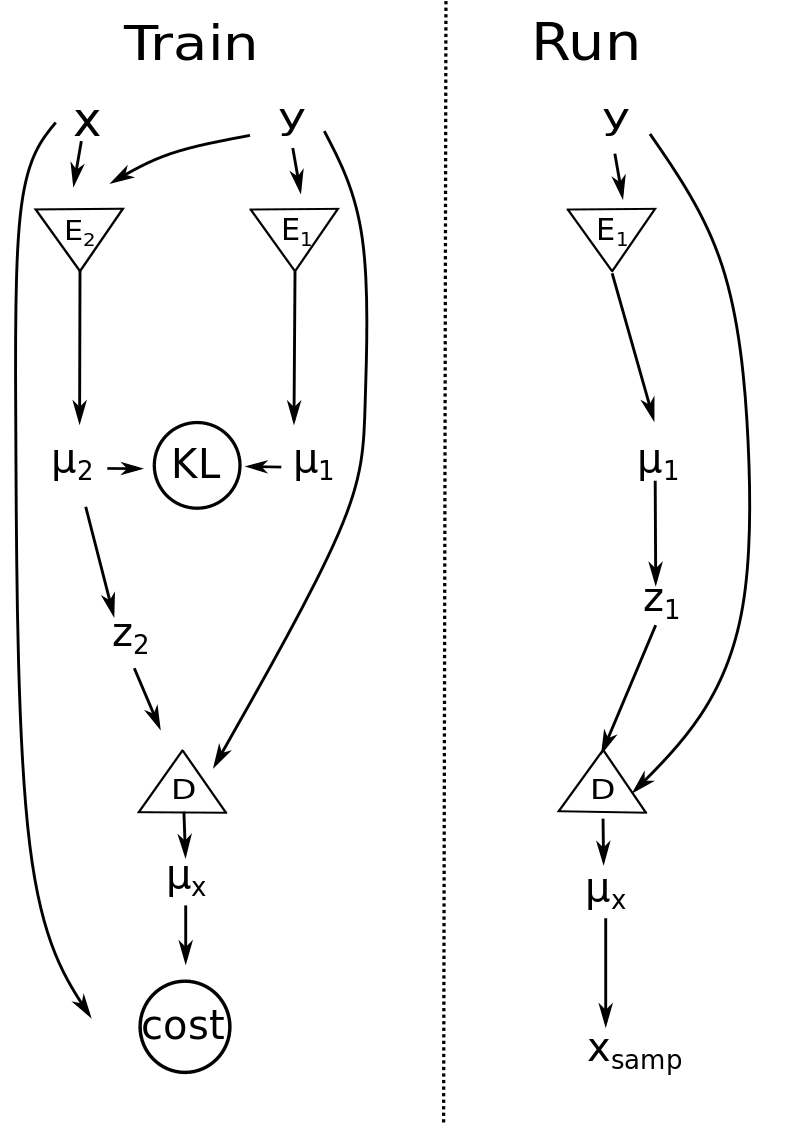
\includegraphics[width=\columnwidth]{images/network_setup.png}
    \caption{\label{fig:network_config}\chris{You are missing a crucial element
here. There should be an arrow from the y data to *both* encoders in the
training. Also, why have we made it so encoder 1 is on the right and encoder 2
is on the left. It reads weird.} This figure illustrates our neural network 
    training/testing operations. During training, a training set of GW signals ($y$) 
    and their corresponding true parameters ($x$) are given as input to encoder 
    networks $\textrm{E}_1$ and $\textrm{E}_2$. The KL divergence (Eq. \ref{eq:kl}) 
    is computed between mean latent space predictions from both encoder networks ($z^1_{\mu},z^2_{\mu}$)
    . $z^2_{\mu}$ is then summed togther with $z_{\log{(\sigma^{2})}} \cdot \epsilon(0,1)$ 
    and given as input to the decoder network. The decoder network predicts $x_{\mu}$ 
    and compares $x_{\mu}$ to the initial training parameters $x$ using Eq. \ref{eq:cost}. 
    After having trained our networks, we test using only $\textrm{E}_1$ and the decoder. 
    A set of test GW signals is given as input to $\textrm{E}_1$ in order to 
    produce a set of $z^1_{\mu}$ predictions. We apply Eq. \ref{eq:z_calc} to 
    get $z$ latent samples. Our $z$ latent space samples are given 
    as input to our decoder network along with our initial test GW signals 
    to get a set of $x_{\mu}$ predictions. We finally apply Eq. \ref{eq:x_calc} 
    to get a set of $x_\textrm{samp}$ samples.}
\end{figure}

%
% Training procedure
%
Training is performed through a series of several steps illustrated in Fig. \ref{fig:network_config}. 
$\textrm{E}_1$ is given a set of training \ac{GW} signals ($y_t$) and encodes $y_t$ into 
latent space $z^{1}_{\mu,\sigma}$. $\textrm{E}_2$ takes a combination of $(x_{t},y_{t})$ 
and is encoded into a latent space described by $z^{2}_{\mu,\sigma}$. 
We then sample from a multivariant Gaussian distrubtion whose mean and standard 
deviation are described by $z^{2}_{\mu,\sigma}$. These samples, along with $y_t$, then go 
to the decoder in order to get out a statistical description of another 
multivariant Gaussian distribution ($x_{\mu,\sigma}$). A cost function is then 
computed between $x_{\mu,\sigma}$ and the corresponding training parameters ($x_t$) and is minimized. 
Essentially, the cost function is used to learn how to predict the
closest value of $x$ (through $x_{\mu}$) and the variation of that $x$ (through
$x_{\sigma}$). Recall that $x_{\mu}$ and $x_{\sigma}$ are not fixed for the
whole dataset - so they're not modelling the spread of $x$ as a multivariate
Gaussian - they have learned the $x_{\mu}$ and $x_{\sigma}$ for any input pair
of $x$ and (crucially) $y$.
Additionally, the K-L divergence between both $z^{1}_{\mu,\sigma}$ and $z^{2}_{\mu,\sigma}$ is 
computed and minimized in order to ensure that both distributions are consistent with each other.

%
% Brief introduction to loss functions used in the neural networks
%
In order for our variational autoencoders to learn anything, we need a metric by which 
we can assess the effectivness of our three networks. This is done by computing 
a loss function which minimizes the difference 
between predictions on the posterior with respect to the truth (cost function) and the Kullback-Leibler divergence 
between latent space distributions $z_1$ and $z_2$. 

%
% Cost function
%
The cost function is constructed by first defining a normalization factor

\begin{equation}
    f_{\textrm{norm}} = 0.5 \cdot \log(c + \exp(x_{\sigma})) - 0.5 \cdot \log(2\pi),
\end{equation}

where $c$ is a small constant and $x_{\sigma}$ are standard deviation predictions 
on the source paramters from the decoder network given latent space predictions 
from encoder-2 ($z_2$) and training GW sigals ($y_{t}$). We then 
compute 

\begin{equation}
    x_{\textrm{diff}} = (x^{z,y}_{\mu} - x_{\textrm{train}})^{2},
\end{equation}

where $x^{z,y}_{\mu}$ are the predicted mean parameters from the decoder network 
and $x_{\textrm{train}}$ are the true training parameters we are 
trying to predict. A Gaussian likelihood is computed and summed over

\begin{equation}
    \textrm{cost} = - \sum (-\frac{x_{\textrm{diff}}}{2c \cdot 
    x^{z^{x,y_{\textrm{train}}}_{\sigma},y_{\textrm{train}}}_{\sigma^{2}}} + f_{\textrm{norm}}),\label{eq:cost}
\end{equation}

where $x^{z^{x,y_{train}}_{\sigma},y_{train}}_{\sigma^{2}}$ are standard deviation squared predictions from the 
decoder network.


%
% KL divergence
%
The K-L divergence is computed in order to train 
encoder-1 and encoder-2 to produce consistant latent space 
distributions. This is done by computing 

\begin{equation}
    \begin{split}
    \textrm{KL-div} = \sum(\log{z^{y}_{\sigma}}-\log{z^{x,y}_{\sigma}} \\
    +\frac{\exp{(\log{z^{x,y}_{\sigma^{2}}+c)}}+(z^{x,y}_{\mu}-z^{y}_{\mu})^{2}}{2*\exp{(z^{y}_{\sigma^{2}}})}
    -\frac{1}{2}),\label{eq:kl}
    \end{split}
\end{equation}

where $z^{y}_{\sigma}$ is the predicted latent space standard deviation from $\textrm{E}_1$, 
$z^{x,y}_{\sigma}$ is the predicted latent space standard deviation from $\textrm{E}_2$, 
$c$ is a small constant, $z^{x,y}_{\sigma^{2}}$ is the predicted latent space 
standard deviation squared from $\textrm{E}_2$, $z^{y}_{\sigma^{2}}$ is the predicted 
latent space standard deviation squared from $\textrm{E}_1$, $z^{x,y}_{\mu}$ is the 
mean latent space from $\textrm{E}_2$ and $z^{y}_{\mu}$ is the mean latent space 
from $\textrm{E}_1$.

The mean of the summation in equation \ref{eq:cost}, $\overline{\textrm{cost}}$, 
is then summed together with the mean of the summation in equation \ref{eq:kl}, 
$\overline{\textrm{KL-div}}$ to 
get our final loss function

\begin{equation}
    \textrm{loss} = \overline{\textrm{KL-div}} + \overline{\textrm{cost}}.
\end{equation}

This loss is then backpropogated through all three networks 
(encoder-1, encoder-2, decoder) and repeated per batch of 
training samples for a pre-defined number of iterations. For our 
purposes, we found that $\sim3\textrm{e}6$ training iterations and 
a batch size of $128$ training samples were sufficient. A total 
of $1\textrm{e}6$ training samples were used. We additionally 
ensure that an inifinite number of noise realizations are effectively employed. This 
is done by adding a new unique set of random whitened noise to noise-free 
versions of our training samples for every new batch that the networks 
see. Each neural network is three layers deep, has $2048$ neurons, a latent 
space size of $64$ with $50\%$ dropout applied to each layer of each network.

%
% loss plot
%
\begin{figure}
    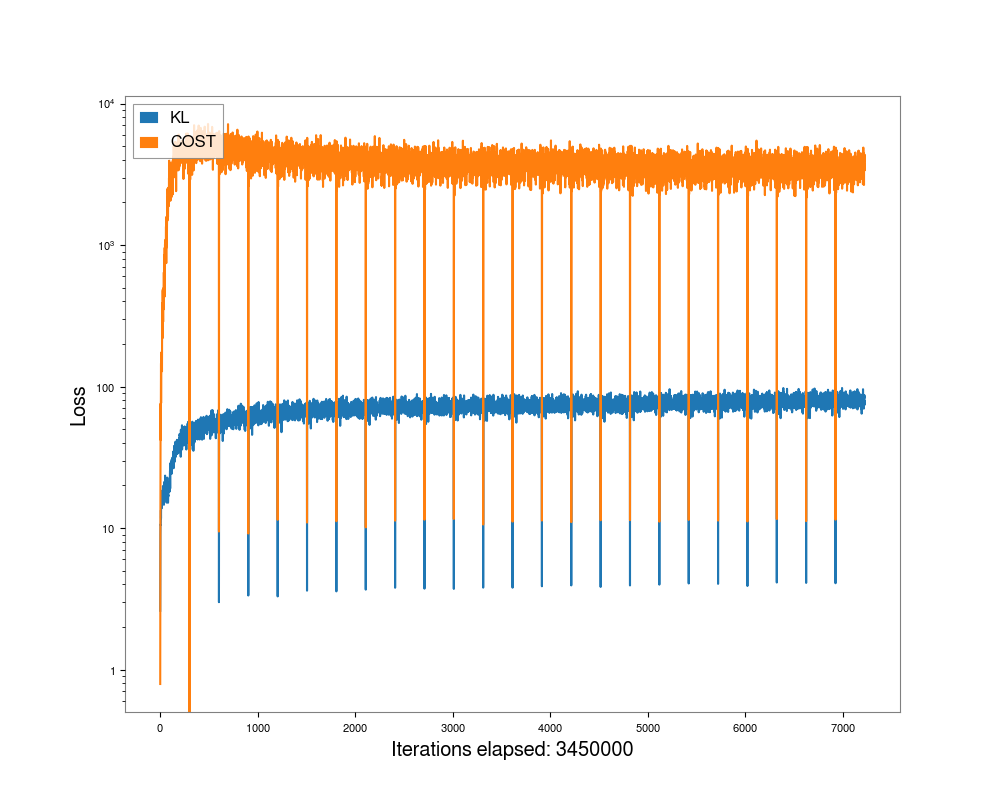
\includegraphics[width=\columnwidth]{images/losses_logscale.png}
    \caption{\label{fig:loss_log} Loss plot with the cost, KL, 
    and total loss values plotted as a function of the total 
    number of training iterations. We can conclude that our 
    neural networks have converged to their optimal state 
    when the slope of our loss curves are close to zero.}
\end{figure}

%
% Test procedure
%
After training has completed, we simply feed encoder-1 our test 
GW signals $y_{test}$. We take the output from encoder-1 $z^{y}_{\mu}$ 
and sample from a univariant Gaussian distribution in order to get 
a set of $z^{y}$ samples. Our $z^{y}$ samples are then combined with our 
test GW signals $y_{test}$ and fed as input to our pre-trained decoder 
network. The decoder network returns a set of mean $x_{\mu}$ predictions 
from which we sample from a Gaussian distribution in order to get 
our final posterior samples.

%
% Results
%
We present results from $25$ test cases of GWs produced from 
a parameter space which is consistent with the prior assumptions  
on the parameter space defined above. The only difference 
being that all of our time of coalescence parameters are fixed 
at $0.5s$ within the $1s$ time window. We compare our 
VAE predictions with posteriors produced by the \texttt{Bilby}
inference library.

%
% K-L divergence results
%
\begin{figure}
    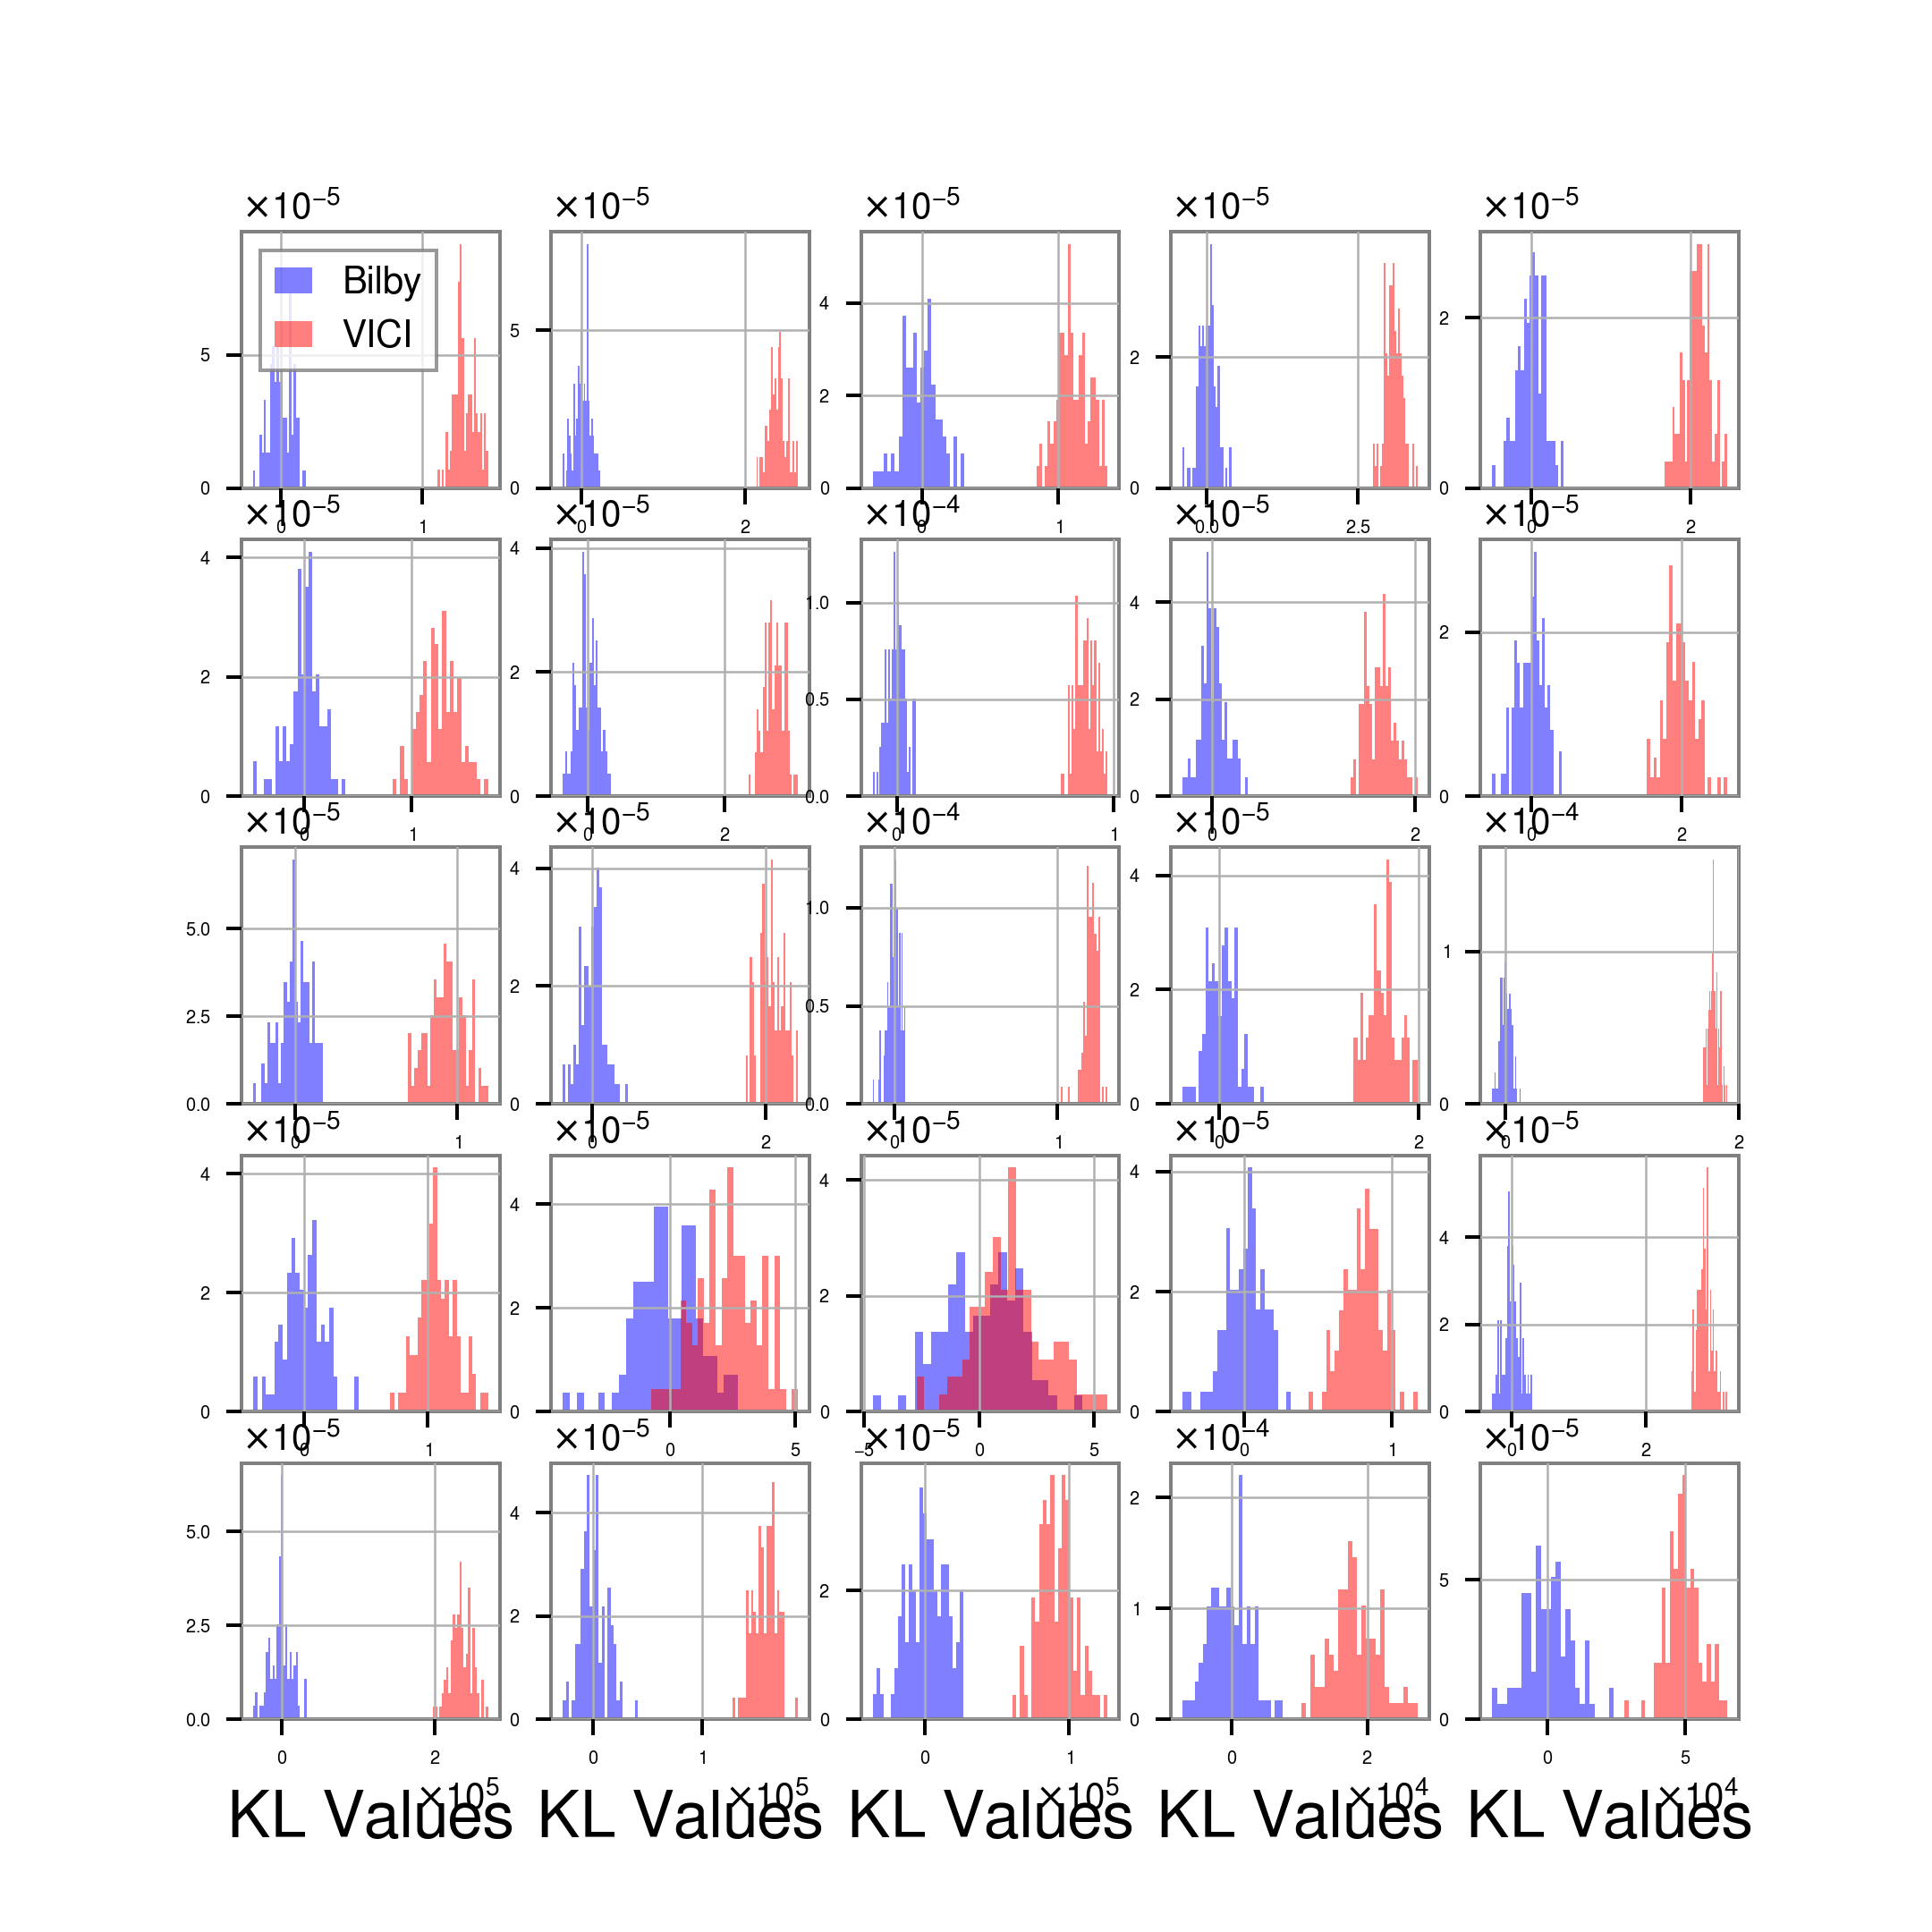
\includegraphics[width=\columnwidth]{images/hist-kl_0.png}
    \caption{\label{fig:kl_results} Histograms of 
    25 different test GW signal KL divergence values. 
    Red denotes predictions from the CVAE and blue 
    denotes predictions from \texttt{Bilby}.}
\end{figure}

In Fig. \ref{fig:kl_results} we show histograms of KL divergence 
values on $25$ test GW samples. The KL divergence is computed 
$100$ times per test sample through the initialization of random splits. We compute 
the KL divergence on CVAE results (red) by comparing CVAE predictions 
to \texttt{Bilby} predictions. Our benchmark \texttt{Bilby} (blue) results are computed by choosing 
random $50/50$ splits between results from the same \texttt{Bilby} produced 
posterior. 


%
% A-D results
%
\begin{figure}
    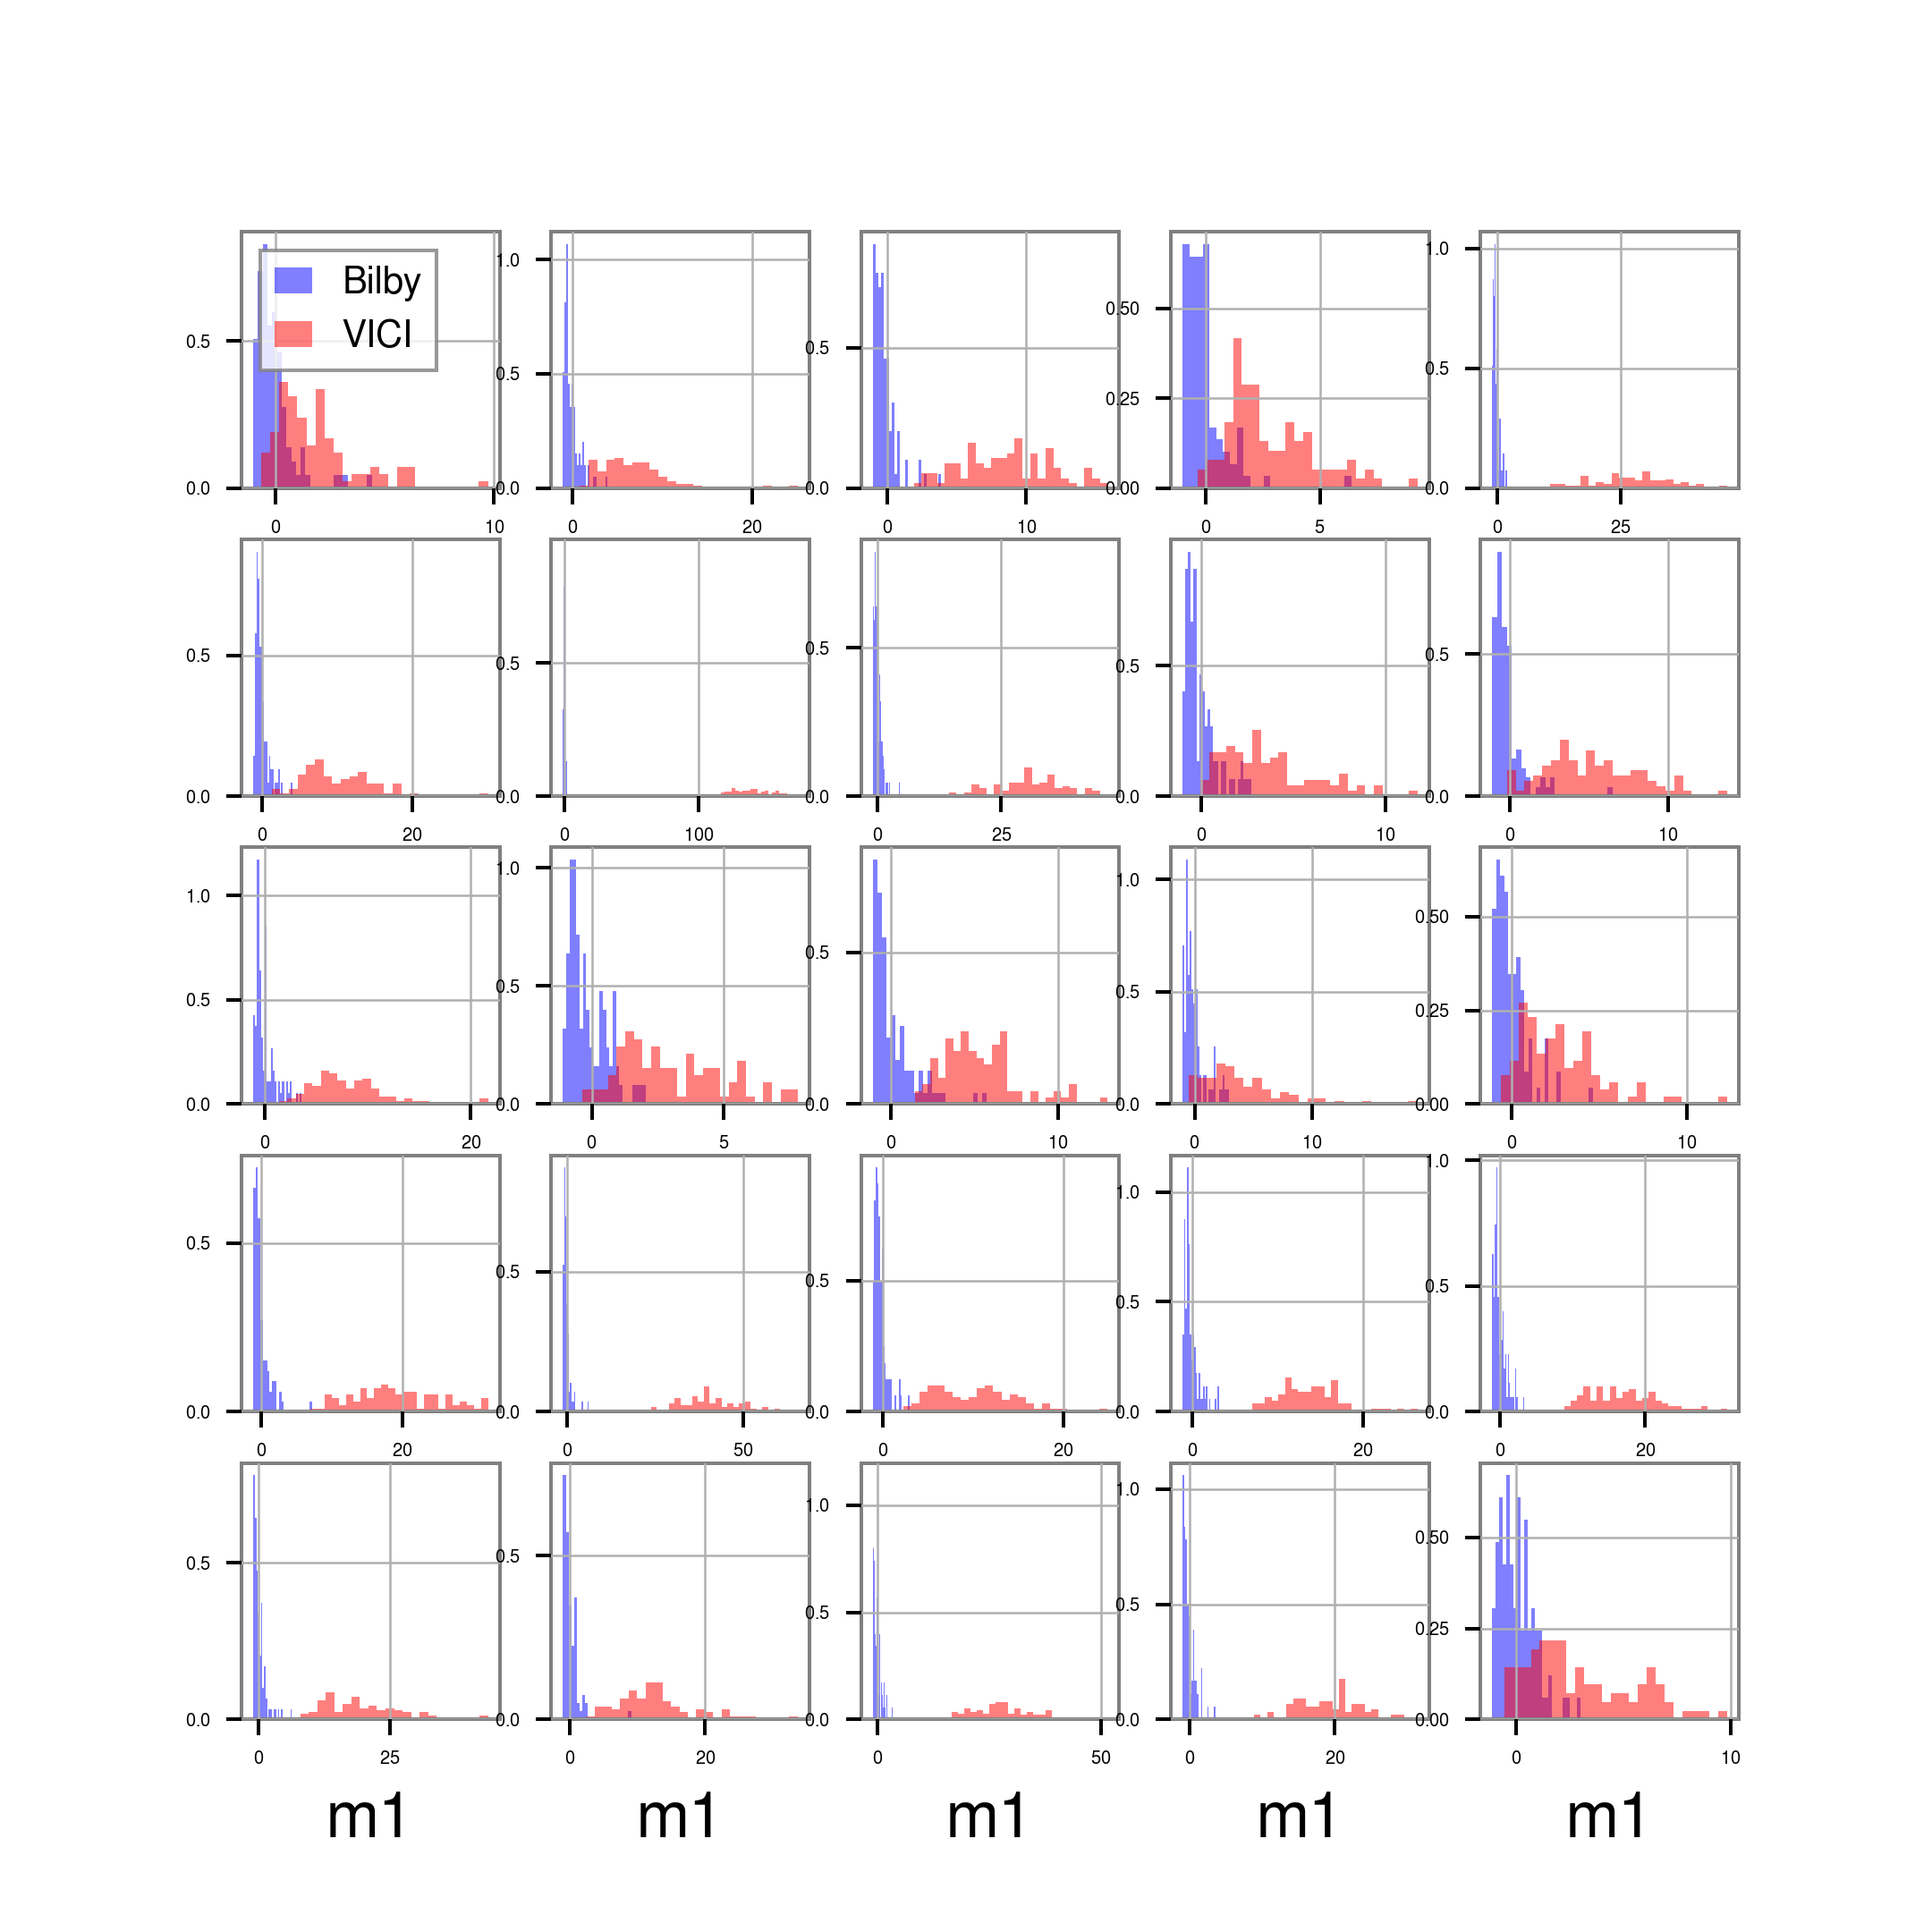
\includegraphics[width=\columnwidth]{images/hist-ad_0.png}
    \caption{\label{fig:ad_results} Histograms of 
    25 different test GW signal Anderson-Darling (AD) statistic 
    component mass 1 values. Distributions which are similar 
    will have AD values which are close to 0.
    Red denotes predictions from the CVAE and blue 
    denotes predictions from \texttt{Bilby}.}
\end{figure}

In Fig. \ref{fig:ad_results} we show histograms of AD 
statistic results computed over $100$ iterations per test sample. 
The AD statistic is a 1-dimensional figure of merit, 
so Fig. \ref{fig:ad_results} only illustrate results 
from predictions on $m_1$. The closer AD statistic 
values are to zero, the more likely that the two 
distributions being compared are drawn from 
the same distribution. As can be seen in Fig. \ref{fig:ad_results} 
there is some overlap between the machine learning 
predictions and our benchmark \texttt{Bilby} results.

%
% P-P plot
%
\begin{figure}
    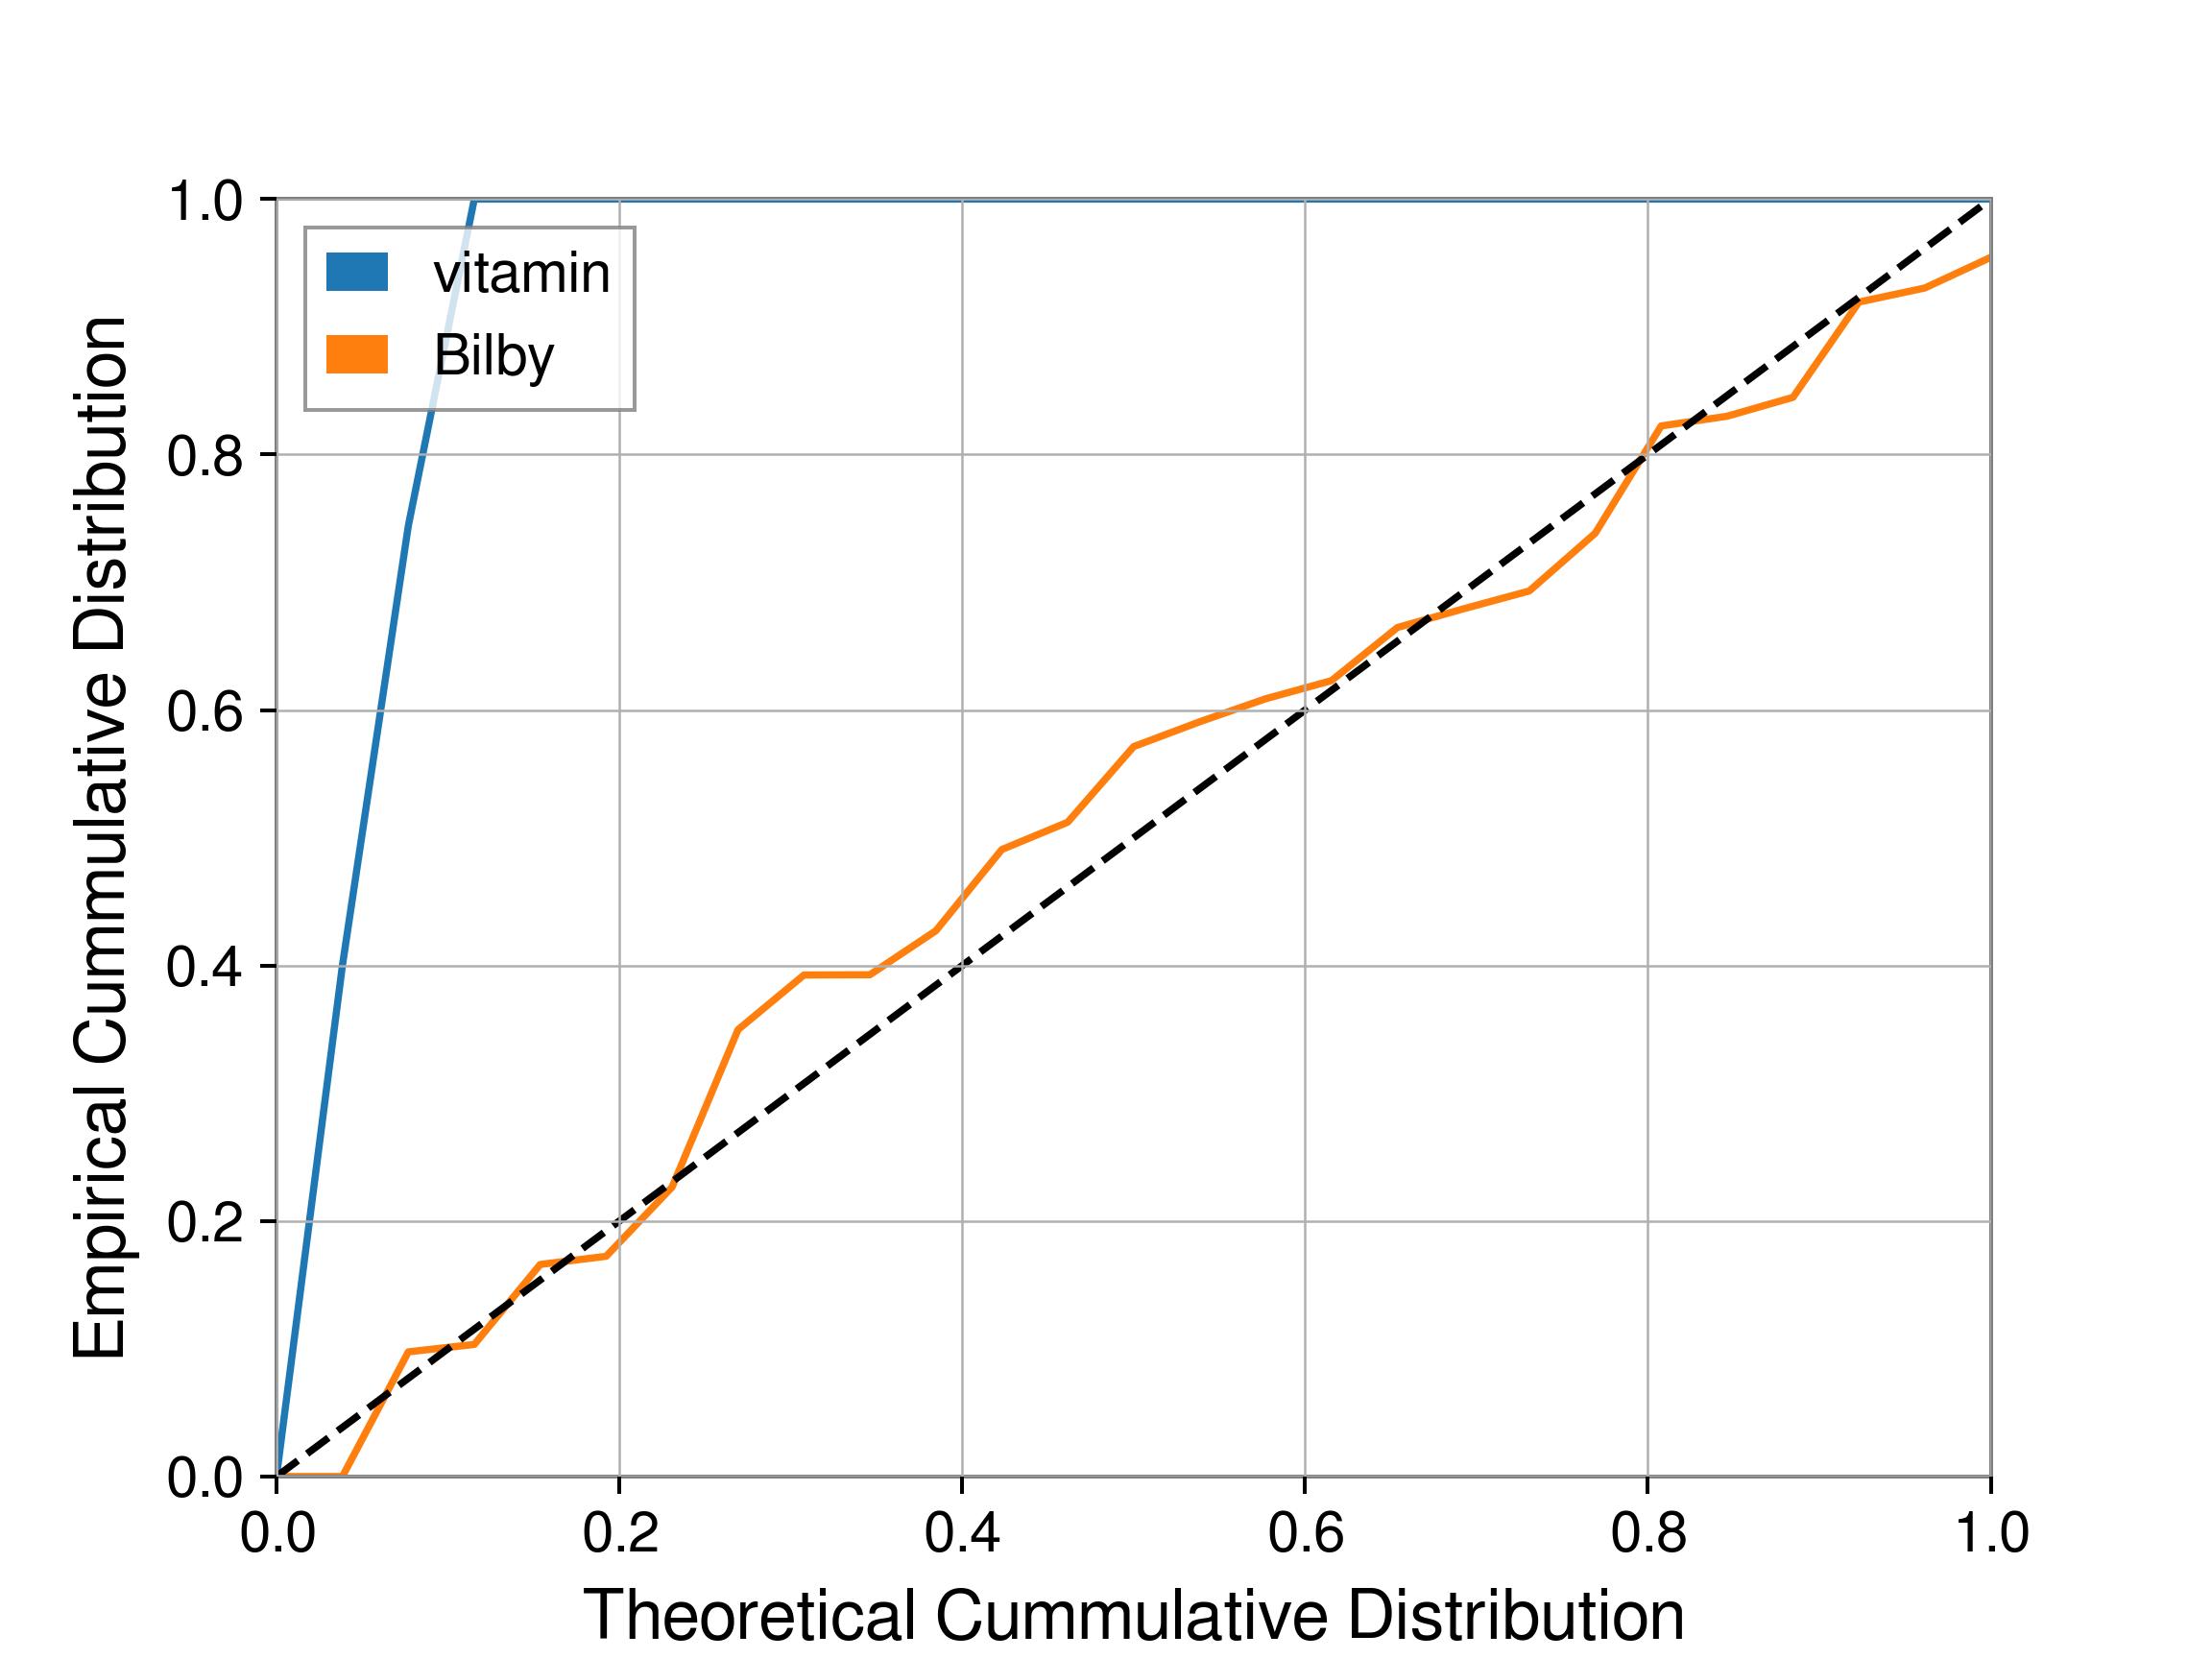
\includegraphics[width=\columnwidth]{images/latest_pp_plot.png}
    \caption{\label{fig:pp_plot} P-p plot 
    using $100$ unique test samples and $5000$
    posterior sample predictions per test sample. 
    The x axis denotes the theoretical cummulative 
    distribution whereas the y axis denotes 
    the predicted cummulative distribution.}
\end{figure}

In order to show that our results are consistent with the 
truth, we have additionally plotted probability-probability (p-p) 
plots in Fig. \ref{fig:pp_plot}. On the y axis is plotted the predicted 
cummulative distribution and on the x axis is plotted the theorectical 
distribution. Perfect alignment with the truth is illustrated by the 
black dashed diagonal line, while our empirical alignment is 
shown in the blue line. 

%
% 1-D overlap results
%
\begin{figure}
    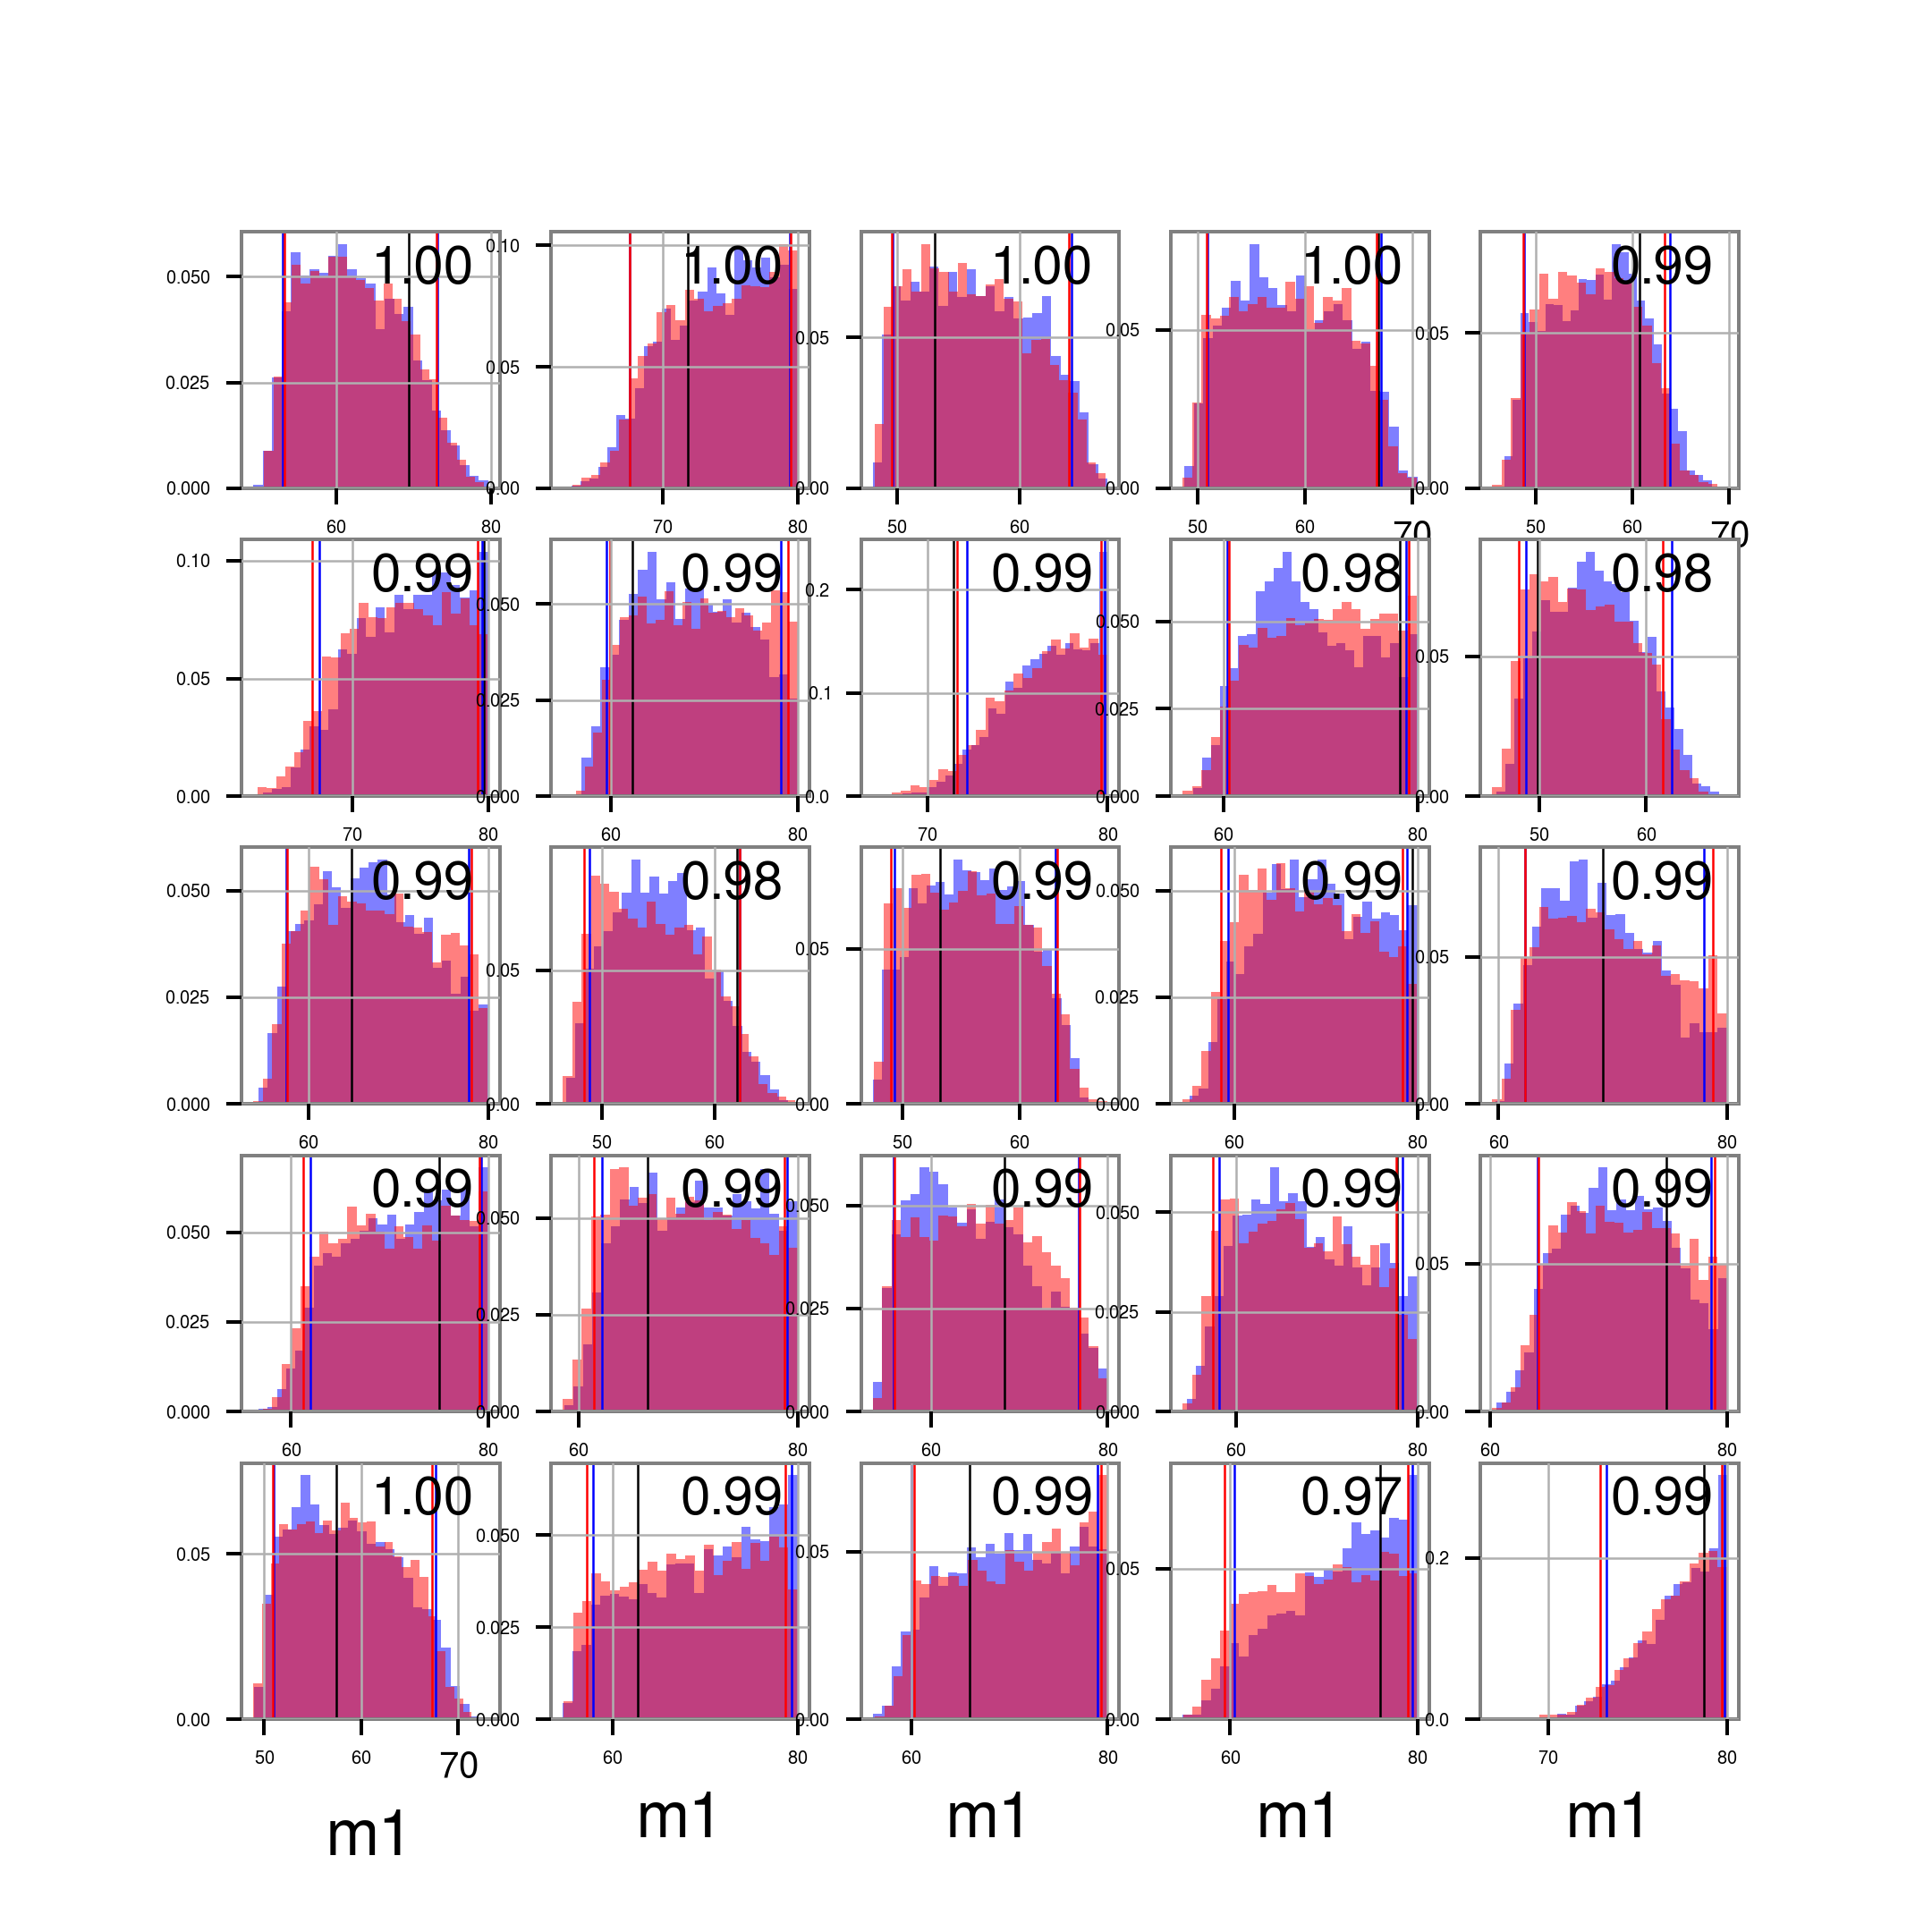
\includegraphics[width=\columnwidth]{images/latest-1d_0.png}
    \caption{\label{fig:1D_overlap} Histograms of 
    25 different test GW signal component mass 1 values. 
    Numbers in the upper right-hand corner denote overlap 
    values where 1 means $\sim{100}\%$ overlap and 0 
    means $\sim{0}\%$ overlap.
    Red denotes predictions from CVAE predictions and blue 
    denotes predictions from \texttt{Bilby}.}
\end{figure}

%
% 2D scatter plot
%
\begin{figure}
    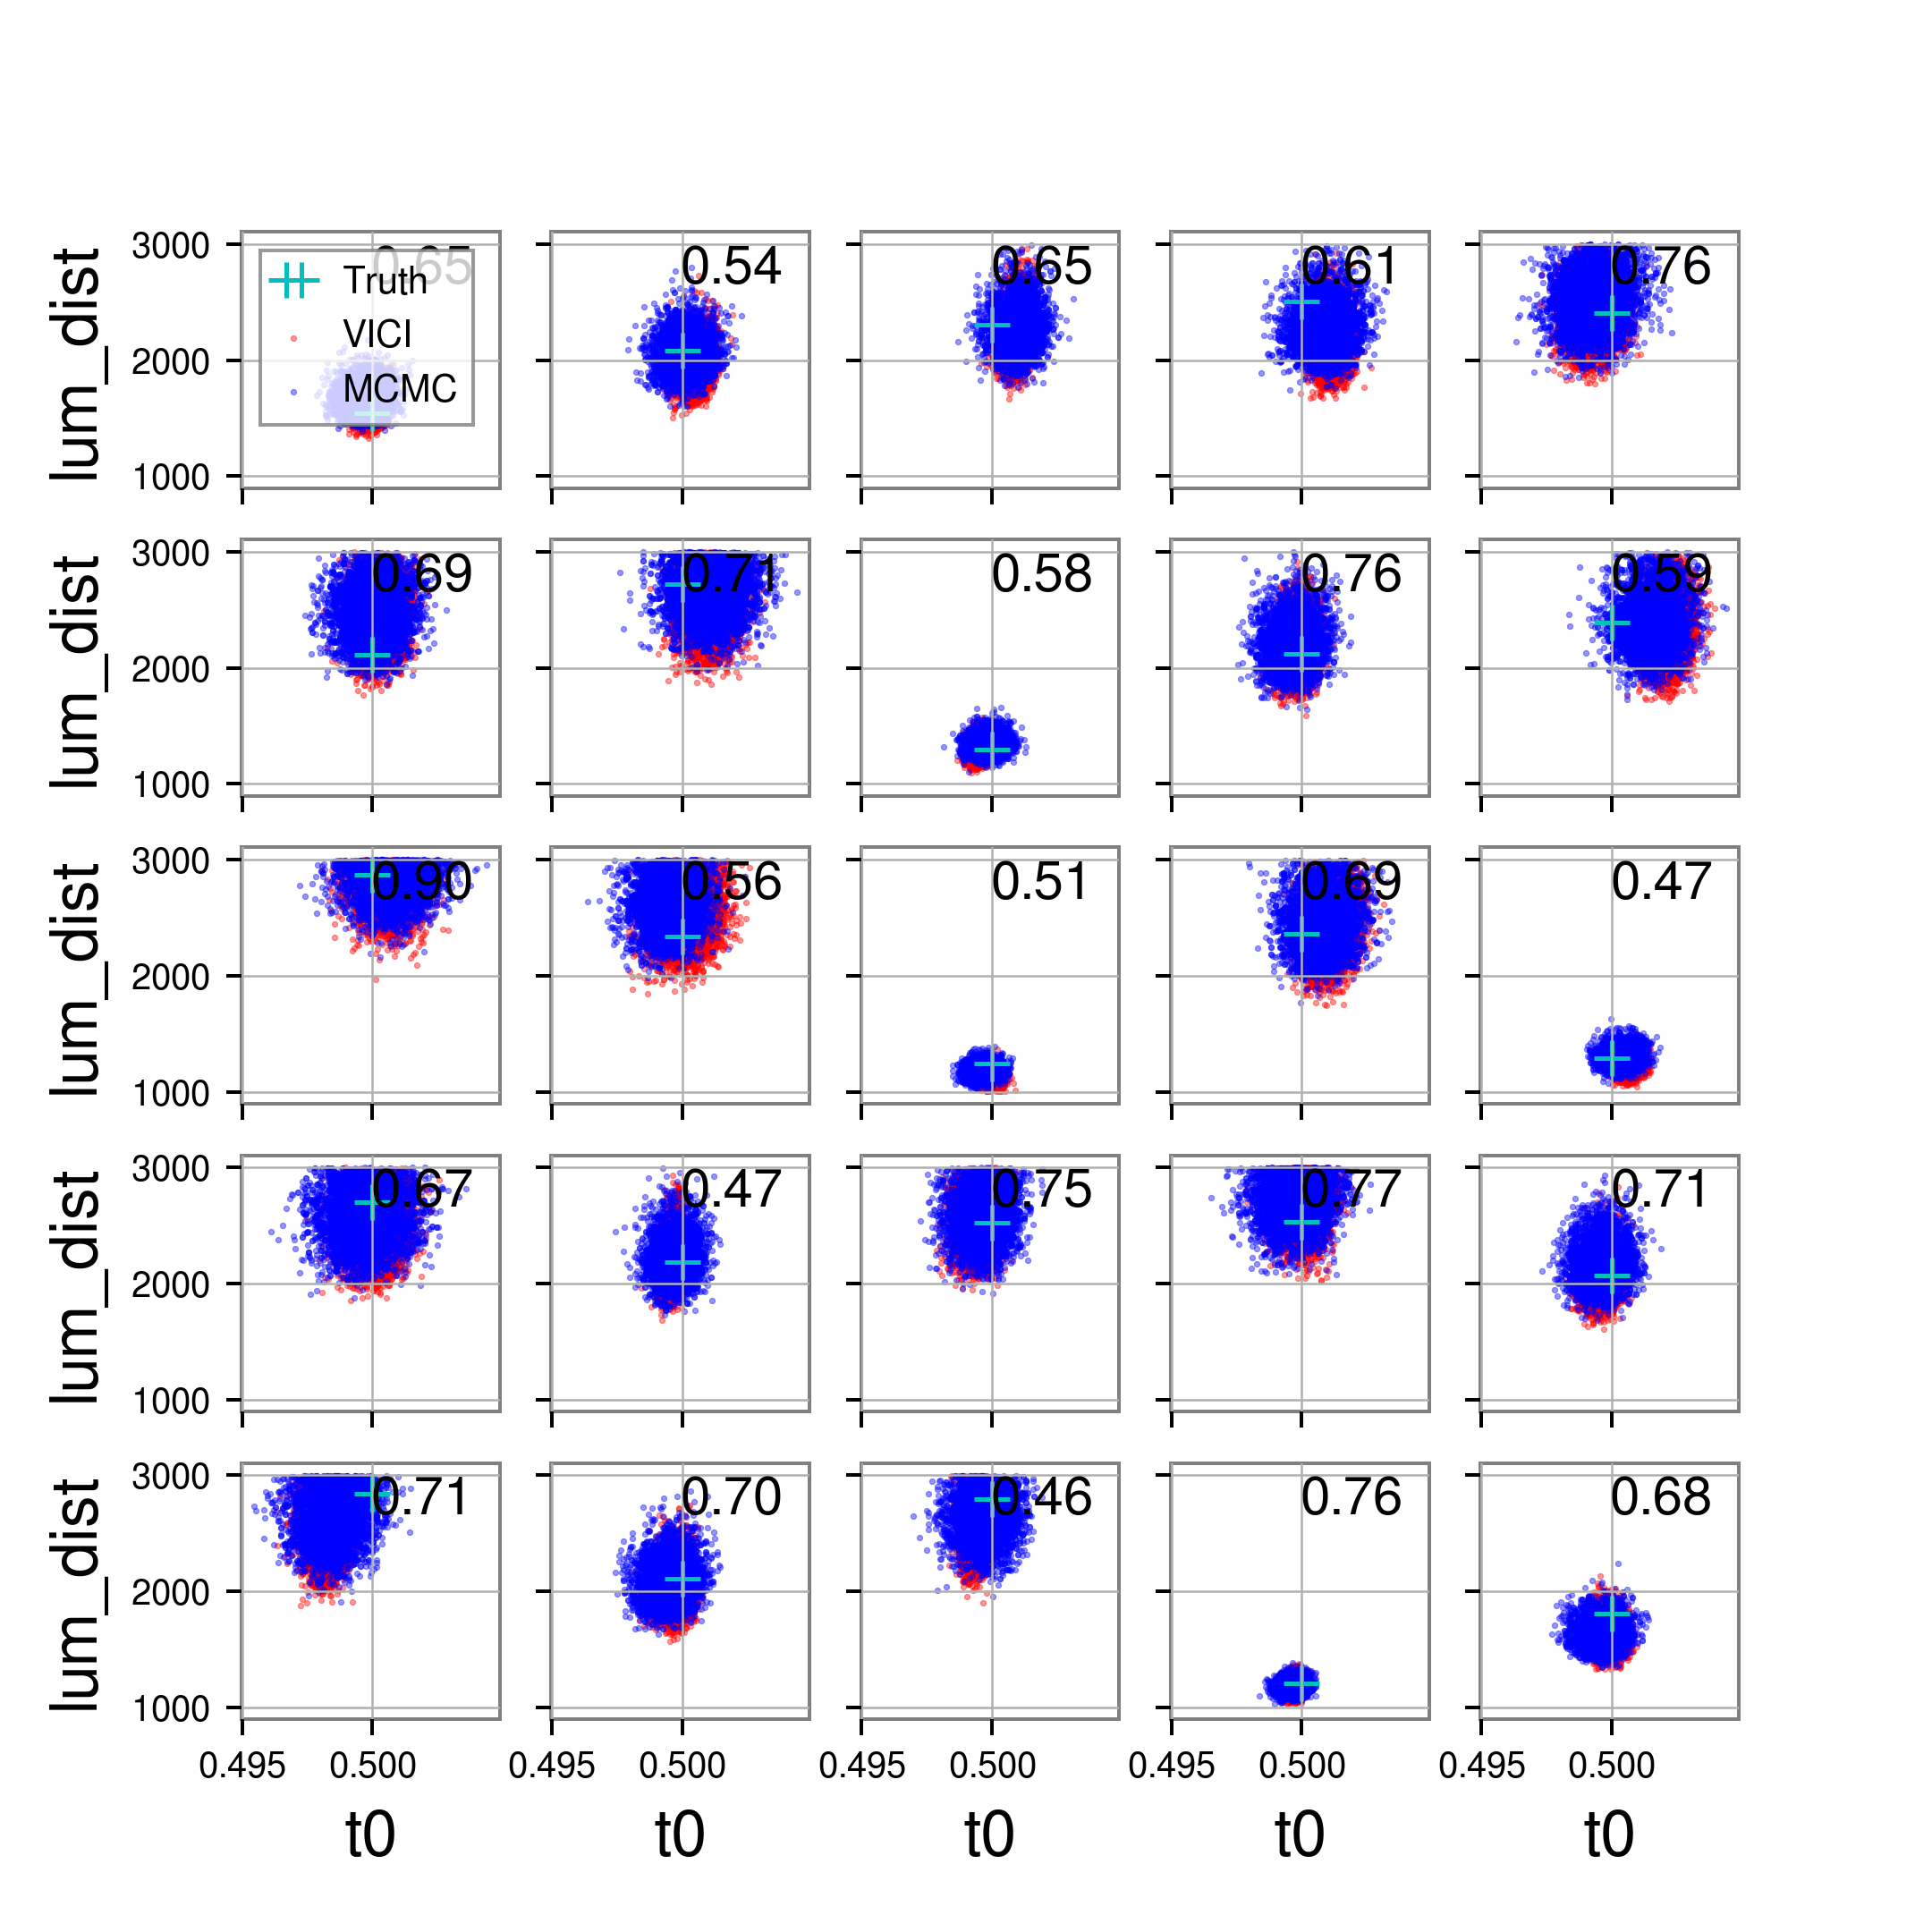
\includegraphics[width=\columnwidth]{images/posteriors_13.png}
    \caption{\label{fig:lum_dist-t0_scatter} This figure illustrates 
    25 different test GW samples with $5000$ posterior samples 
    from both \texttt{Bilby} and our CVAE plotted. Red denotes predictions 
    from the CVAE and blue denotes predictions from \texttt{Bilby}. Luminosity 
    distance is plotted as a function of time of coalescence with 
    4-dimensional overlap values printed in the upper right-hand 
    portion of each subplot.}
\end{figure}

We can further illustrate the accuracy of our machine 
learning predictions by directly plotting the samples 
generated by our CVAE and \texttt{Bilby} superimposed on each other. 
In Fig. \ref{fig:1D_overlap}, we histogram predictions sampled 
from the posterior through both \texttt{Bilby} (blue) and our CVAE (red). 
As can be clearly seen, the overlap between both \texttt{Bilby} and 
the CVAE is extremely high in the $m_1$ parameter space. Additional 
proof of high overlap between posteriors can also be seen 
in Fig. \ref{fig:lum_dist-t0_scatter} where 
we plot samples from both \texttt{Bilby} (blue) and the CVAE (red) posteriors 
with luminsoity distance as a function of $t_0$. 

%
% Conclusions
%
In this letter we have demonstrated that we 
are able to reproduce, to a high degree of accuracy, posteriors 
generated from Bayesian inference using machine learning. This 
is accomplished through the use of variational autoencoders 
trained on over 1 million whitened simulated gravitational 
wave signals. By building a neural network model which, 
when trained, can reproduce the true posterior in less than a 
second, we have demonstrated that neural networks 
can achieve the same sensitivity as that of Bayesian 
inference.

The significance of achieving similar sensitivities 
to Bayesian inference is most evident in the 
orders of magnitude speed-up in performance. The increase
in speed will help the LIGO-Virgo-Kagra calibration 
alert our electromagnetic follow-up partners with 
minimum latency.

Our work can further be expanded upon by including 
a variety of other GW sources such as Neutron star - 
black hole (NSBH) and binary neutron star (BNS) mergers 
at higher sampling frequencies. We have yet to demonstrate 
the effectivness of our method on additional parameters 
such as sky location and inclination angle, the benefits of which 
would be best realized in an end-to-end inference pipeline. 
Such a pipeline would be of great importance as the detectors 
increase up to their full potential design sensitivities.

\section{Methods}
Put methods in here.  If you are going to subsection it, use
\verb|\subsection| commands.  Methods section should be less than
800 words and if it is less than 200 words, it can be incorporated
into the main text.

\subsection{Whitening}

In order to ensure 
that there is equal power accross all
frequency bins of our signal, we ensure that the noise is whitened Gaussian
noise. We whiten using a single detector (H1) power spectrum density derived from the
Advanced LIGO design sensitivity curves \cite{2016LRR....19....1A}. 

\subsection{Nested Sampling}
%
% Describe nested sampling algorithm
%
If we would like to find the results for a particular parameter, 
we simply marginalize over all unwanted parameters 

\begin{equation}
    p(x_1|y) = \int dx_2 ... dx_N p(x|y).
\end{equation}

There are several algorithms which may be used to sample from the posterior
distribution of astrophysical GW source parameters \cite{PhysRevD.64.022001,
skilling2006,10.1111/j.1365-2966.2011.20288.x}. The
algorithm which is used in our case is the nested sampling algorithm. Nested
sampling takes a multi-dimensional evidence integral calculation (fully
marginalized likelihood) and transforms it into a more manageable 1-D integral
, where evidence is the integral of the likelihood 
multiplied by the prior over all parameters of the model $H$ ~\cite{1409.7215}

\begin{equation}
    Z = p(y|H) = \int dx_1 ... dx_n p(y|x,H)p(x|H).\label{eq:evidence}
\end{equation}

%
% More nested sampling description
%
The first step of the nested sampling algorithm starts by generating an initial
set of live points made from the prior distribution. The likelihood for each
point is calculated and the point with the lowest likelihood is removed. The
removed sample is then replaced with a new sample which has a higher
likelihood. This cycle repeats itself until a predefined stopping threshold is
achieved \cite{1409.7215} . Samples from the posterior may be drawn by randomly
selecting from both all current 'live' points and all previously removed 'live'
points.

The nested sampling algorithm is run using
1000 live points and has a predefined stopping criteria of $0.1$~\chris{expand
upon what the stopping criteria means. This is related to the evidence
calculation and the tolerance on that result}. The sampler takes $\mathcal{O}(3
\: \textrm{minutes})$ to converge~\chris{jargon. What does converge mean to the
average Nature reader?}. After the nested sampler has converged~\chris{jargon}, we draw
samples~\chris{too technical with not enough explanation. The \texttt{Bilby} analysis
produces posterior parameter estimates and does so by supplying the user with
samples drawn from that distribution.} and produce a posterior on the
astrophysical \ac{GW} source parameters we are trying to estimate.

%
% acknowledge peopkle and funding agencies
%
\section{Acknowledgements.}
%
We would like to acknowledge valuable input from the LIGO-Virgo Collaboration
specifically from {\textbf{someone}}, and the parameter estimation and
machine-learning working groups. The authors also gratefully acknowledge the
Science and Technology Facilities Council of the United Kingdom. CM is
supported by the Science and Technology Research Council (grant
No.~ST/~L000946/1).

%% Here is the endmatter stuff: Supplementary Info, etc.
%% Use \item's to separate, default label is "Acknowledgements"

%\begin{addendum}
% \item Put acknowledgements here.
% \item[Competing Interests] The authors declare that they have no
%competing financial interests.
% \item[Correspondence] Correspondence and requests for materials
%should be addressed to Hunter Gabbard~(email: h.gabbard.1@research.gla.ac.uk).
%\end{addendum}

\bibliographystyle{apsrev4-1}
\bibliography{references}% Produces the bibliography via BibTeX.

\end{document}
